\clearpage{\pagestyle{empty}\cleardoublepage}
\chapter{Introduzione al fotovoltaico}
%
L'\emph{effetto fotovoltaico} consiste nel passaggio di elettroni 
dalla \emph{banda di valenza} alla \emph{banda di conduzione} di 
un materiale, a causa dell'assorbimento di \emph{fotoni}. 
%
Tale fenomeno viene sfruttato dai \emph{moduli (o celle) fotovoltaici}, 
allo scopo di trasformare l'energia contenuta nella radiazione luminosa 
in energia elettrica.
%

%
\section{I moduli fotovoltaici}
I moduli fotovoltaici costuiscono gli elementi base di ogni impianto
fotovoltaico. Si tratta di dispositivi costituiti da \emph{fette} di 
materiale \emph{semiconduttore}. L'utilizzo dei semiconduttori \`e 
fondamentale, per via del loro caratteristico \emph{band gap}, di 
dimensioni tali per cui \Item{i} gli elettroni riescono facilmente 
a passare dalla banda di valenza a quella di conduzione a seguito 
dell'apporto energetico fornito dalla radiazione luminosa, \Item{ii} 
gli elettroni che effettuano il passaggio nella banda di conduzione 
non vengono neutralizzati.
%

%
La presenza di \emph{portatori di carica} nella banda di conduzione 
fa si che il modulo fotovoltaico, una volta connesso ad un 
conduttore esterno, si comporti come un 
\emph{generatore di corrente}\cite{bellini09}.
%
\begin{figure}[!h]
\centering
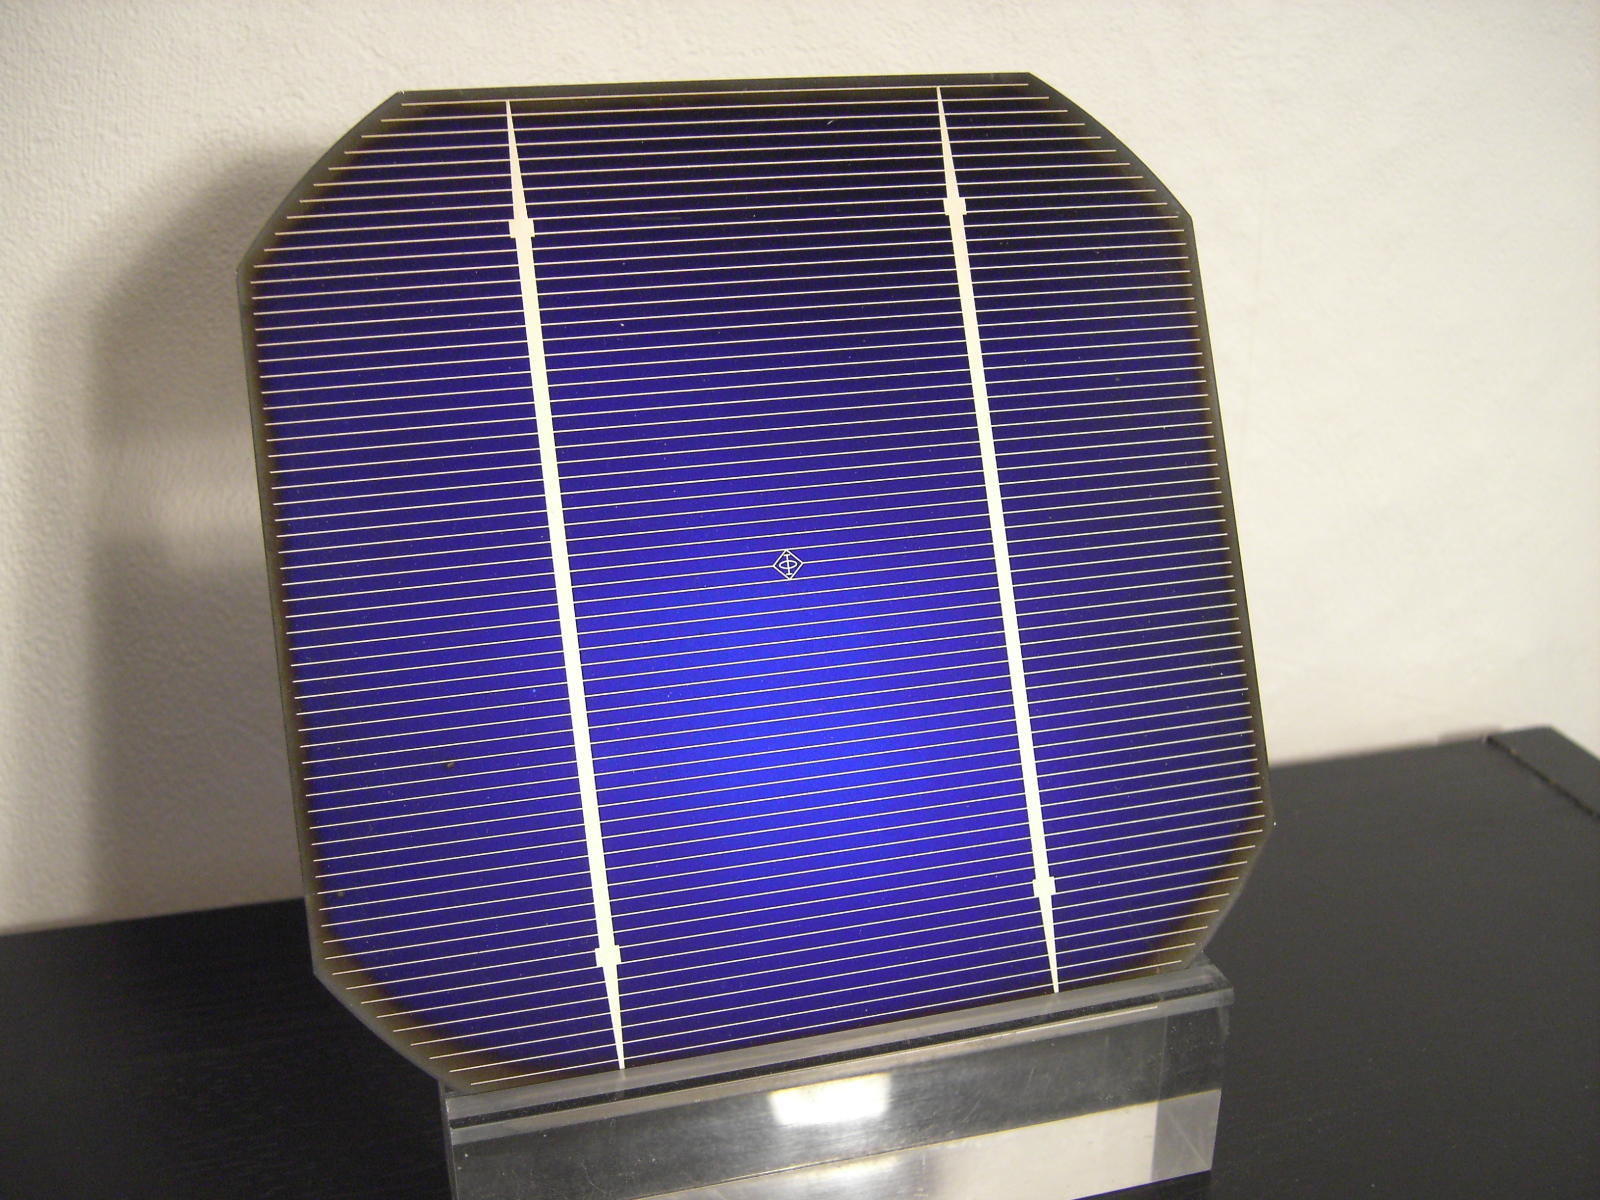
\includegraphics[width=350pt]{img/modulo-fotovoltaico.jpg}
\caption{Modulo fotovoltaico in silicio \emph{monocristallino}}
\end{figure}
%
Allo stato attuale, esistono diverse tecnologie di realizzazione di 
moduli fotovoltaici, la maggior parte basate su processi al silicio.









%% architettura tipica di un impianto fotovoltaico
%% quali informazioni si vogliono produrre?
%% quali informazioni e` necessario rilevare?
%% lista dei desiderata per un sistema di monitoraggio
